\chapter{Fundamentals of Electric circuits}

In this chapter, a method is defined that is used to develop mathematical models to capture the dynamic behavior of electrical systems.

\section{Basics of Electricity}

A particle can either have a positive charge or a negative charge. Like charges repel and unlike charges attract each other. This is because charged particles creates an electric field as shown in figure \ref{Fig_FundElk_01} and an electric field in turn exerts a force on charged particles as shown in figure \ref{Fig_FundElk_02}.
\begin{figure}[h!]
	\centering
	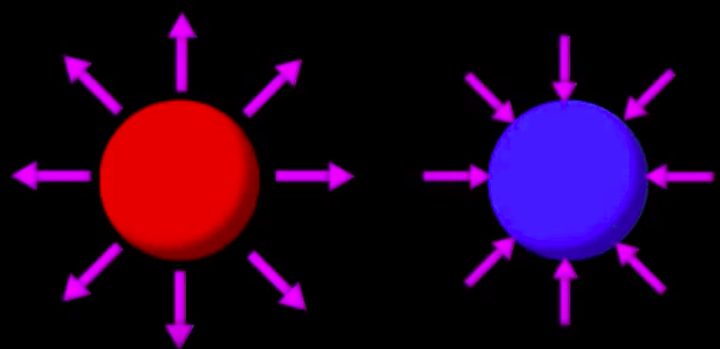
\includegraphics[width=0.5\linewidth]{Bilder/FundElk01}
	\caption{Charged particles creates electric fields}
	\label{Fig_FundElk_01}
\end{figure}
\begin{figure}[h!]
	\centering
	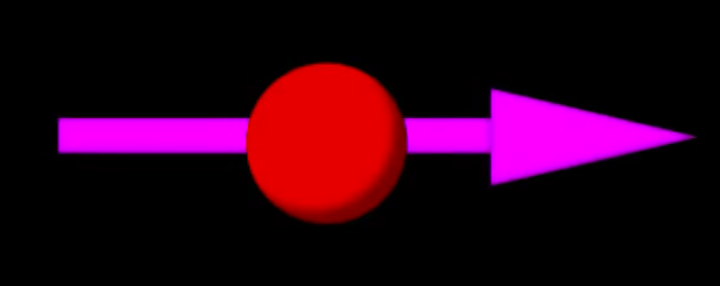
\includegraphics[width=0.5\linewidth]{Bilder/FundElk02}
	\caption{Electric fields exert force on charged particles}
	\label{Fig_FundElk_02}
\end{figure}

When there is an electric field between two points, it is said that there is a \textbf{\textit{voltage}} between these two points. A voltage difference in practice creates this electric field between two points in space through use of devices such as batteries. The electric field then exerts a force on the charged particles that move around because of it. The number of flow of the charged particles in called the \textbf{\textit{current}} in the circuit.

A voltage difference between any two points essentially acts like a potential difference due to height in a gravitational field. Where the height will be the voltage and the gravitational field will be electric field. With one difference that in case of electric circuits higher voltage difference will cause a stronger electric field and vice-versa. The current is a flow-rate of charged particles and therefore can be denoted by $I  = dq/dt = \dot{q}$. Voltage is the potential energy every charged particle and is denoted using either $V$ or $e$ in this notes. Therefore, if we need to get the total power from the circuit the charge flow-rate can be multiplied with the energy of the each charge $(e)$. $$ P = \dot{q} e $$

\textbf{Tip}: The circuit already has the charged particles in it, a battery only creates an electric field (by imposing voltage between two points) which pushes the charged particles along the circuit. Also in the olden times, current was thought to be the flow of positive charged particles, however, it has been found  that it is the electrons that flow in the circuit.

Only a moving charged particle creates a \textbf{\textit{magnetic field}}. And the magnetic field is exerted only on other moving charged particles. A charged particle moving in a loop creates a magnetic field that loops from north pole to the south pole of the charged particle which is same as a single electric charge spinning. A \textbf{\textit{magnet}} is an object where all such spinning charged particles are all moving collectively in the same direction. Therefore, creating a magnetic field that loops from north pole to the south pole. The property of a charged particle to create both electric and magnetic fields is called \textbf{\textit{electro-magnetic}} property, this principle is used in design of electro-magnetic sensors and actuators (DC Motor).

\section{Modeling Electrical System}

Similar to mechanical systems, electrical systems are of three basic types:
\begin{enumerate}
	\item Resistance elements -- Dampers elements
	\item Capacitance elements -- Spring elements
	\item Inductance elements -- Inertia elements
\end{enumerate}

\textbf{Resistance Elements}

Resistance elements are modeled using Ohm's law which states that the voltage drop across the resistor as follows (here current is denoted using $i$):
\begin{equation}
	e = i R
\end{equation}

\textbf{Capacitance element}

The voltage across a capacitor is expressed using the definition of capacitance, which says that the capacitance of a capacitor is equal to the charge stored by the capacitor per unit of voltage supplied to it. Therefore, capacitance $C$ can be defined as:
\begin{equation}
	C = \frac{q}{e}
\end{equation}
the voltage equation can then by written as:
\begin{equation}
	e = \frac{1}{C} q
\end{equation}
Capacitor stores potential energy just like a spring, when voltage is applied to capacitor it holds a charge inside which is then released to the circuit after removing the voltage across the capacitor. 

\textbf{Inductance element}

An inductor acts like an inertia elements of a mechanical system. As inertia of a object due to its mass or shape resists a change in the direction of the motion, here a magnetic field does this to an electrical circuit. Magnetic fields are generated in an electrical circuit when there is a change (magnitude or direction) in electric field. These magnetic fields acts like an inertia to the change in electric field. An electric in this sense is the magnitude of current $i$ and its direction giving in essence the nature of electric field. Similar to a rotating mass which tries to maintain the rotation in the same magnitude and direction. A magnetic field which will be generated again when the current $i$ in the circuit changes its magnitude or direction. This magnetic field will then provide resistance to the electric field (current $i$ and its direction) to be changed. Also noting that whenever there is not change in the electric field, the magnetic field is not generated and the inductor will just behave like a wire allowing all the current to flow through it.

Inductance as its is related to a phenomenon like inertia in mechanical systems is something which stores kinetic energy of the electric circuit. The voltage across an inductor is expressed as a function of change in $i$:
\begin{equation}
	e = L \frac{di}{dt}
\end{equation}
The above equation can be verified using two observations:
\begin{itemize}
	\item When there is a change in $i$, the voltage drop occurs as the function of the change (slope $di/dt$)
	\item When there is no change (slope = 0), then voltage drop across inductor is zero and it behaves just like a wire
\end{itemize}

\section{Principles of electrical systems}

Once the fundamental principle of basic forms of electrical components has been established, the established laws of electrical circuits are used to model the behavior of the dynamical system. There laws are called \textbf{\textit{Kirchhoff law's}} which in essence are like Newton's laws required to model the dynamics of mechanical system. There are two law's of Kirchhoff for electrical circuits:

\subsection{Kirchhoff's Laws}

\textbf{Current Law}
States that the sum of currents $i$ entering any node should be exactly equal to the sum of $i's$ leaving that node.

\textbf{Loop Law}
States that the sum of voltages around the loop should be zero

Using these two laws any electric circuit can be modeled. In case of electric circuits it is rather quite simple to model then as there are only two laws that govern their dynamic behavior. Unlike in mechanical systems there are laws differently stated and for liner and rotational motions, further getting complex when there is addition of constraints into the system.

\subsection{Modeling electrical circuits}

\textbf{Resistors in series}

The voltage applied across resistors in series drops after every resistor as it is a potential energy of the charge which drops off at different levels of energy states. At each energy state that is in this case a resistor the voltage drop across all such elements can be described using Ohm's law such that $e_i = i R_{i}$. Further, applying Kirchhoff's laws, as the current entering the node should be equal to the current leaving the node, the current across every resistor is same. This is also evident from Ohms law $e = i R$, as $R$ changes, voltage drop $e$ changes accordingly and $i$ is a constant in this equation.

\begin{figure}[h!]
	\centering
	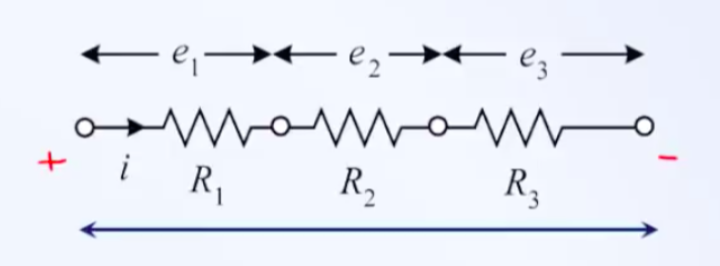
\includegraphics[width=0.75\linewidth]{Bilder/Fund_ELK_SeriesRest}
	\caption{Resistors in series}
	\label{Fig_Fund_ELK_SeriesRest}
\end{figure}

Only using the first law, the dynamic behavior can be modeled as:

\begin{figure}[h!]
	\centering
	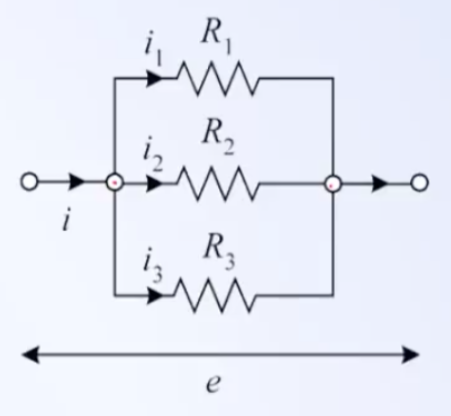
\includegraphics[width=0.75\linewidth]{Bilder/Fund_ELK_ParelRest}
	\caption{Resistors in parallel}
	\label{Fig_Fund_ELK_ParalRest}
\end{figure}

\begin{equation}
	e = i R_1 + i R_2 + i R_3 = i (R_1 + R_2 + R_3)
\end{equation}

\textbf{Resistors in parallel}

Only using the first law the system can be modeled again as with resistors connected with series, the current splits at the node where the connections split into three. Therefore, now the voltage drop across different resistors is given by $i_1 R_1$, $i_2 R_2$ and $i_3 R_3$. However, the voltage across each resistor is same, therefore the system can be modeled as follows:
\begin{equation}
	\sum i = i_1 + i_2 + i_3 = \frac{e}{R_1} + \frac{e}{R_2} + \frac{e}{R_3}
\end{equation}

\subsection{Modeling DC converter}

There are two types of DC converters, voltage amplifiers (boost converters) and voltage attenuators (buck converters). The boost converter is as shown in figure \ref{label}. There are two states in the circuit, ON state and OFF state. The idea is to use the flow of the current is the circuit is such as way that when the current flows into the battery that needs to be charged at higher voltage gets this higher voltage due to the flow of current in te circuit. In ON states when the switch is ON, the current only flows in the first loop through the inductor, as inductor will try to hold the current in the circuit when the switch in is the OFF state, the second loop is activated where now the initial current $i \neq 0$. The task is to find out using Kirchhoff's law for circuits weather the voltage has been stepped up due to such non zero initial current into the circuit.

\begin{figure}[h!]
	\centering
	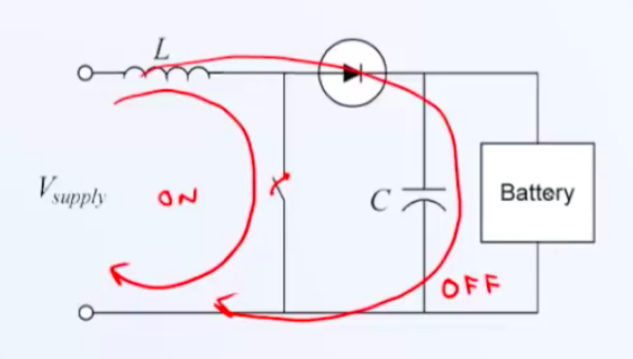
\includegraphics[width=0.75\linewidth]{Bilder/Fund_ELK_Boost}
	\caption{Schematic of a boost converter}
	\label{Fig_Fund_ELK_Boost}
\end{figure}

\textbf{ON State}

\begin{figure}[h!]
	\centering
	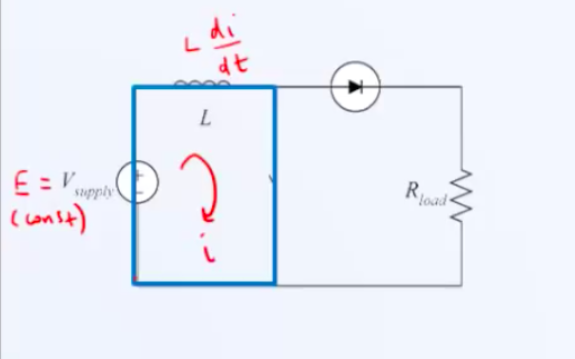
\includegraphics[width=0.75\linewidth]{Bilder/Fund_ELK_Boost_ON}
	\caption{Boost converter CKT in ON mode}
	\label{Fig_Fund_ELK_Boost_ON}
\end{figure}

Using second law and applying at a point (generally any point can be chosen in the ckt):
\begin{equation}
	V_{supply} - L \frac{di}{dt} = 0
\end{equation}

Applying LT for the above equation:
\begin{equation}
	\frac{E}{s} - L (sI(s) - i(0)) = 0
\end{equation}
As $i(0) = 0$, the initial condition, $$ \frac{V}{s} - L (sI(s)) = 0 $$ the current $I(s)$ is:
\begin{equation}
	I(s) = \frac{E}{L}\frac{1}{s^2}
\end{equation}
inverse LT on the above equation:
\begin{equation}
	i = \frac{E}{L} t, \quad t \geq 0 \label{Eq_Fund_Elk_Boost_ON}
\end{equation}

\textbf{OFF state}

\begin{figure}[h!]
	\centering
	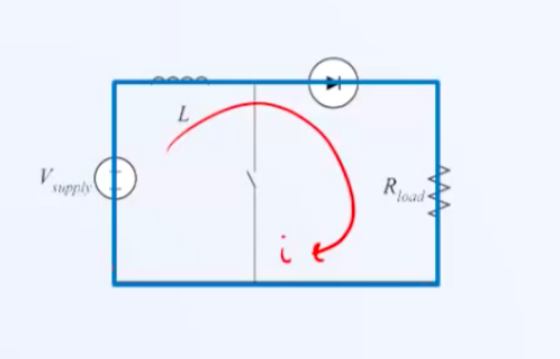
\includegraphics[width=0.75\linewidth]{Bilder/Fund_ELK_Boost_OFF}
	\caption{Boost converter CKT in OFF mode}
	\label{Fig_Fund_ELK_Boost_OFF}
\end{figure}

\begin{equation}
	V_{supply} - L \frac{di}{dt} - R_{load} i = 0
\end{equation}

applying LT:

\begin{equation}
	\frac{E}{s} - L (sI(s) - i(0)) - R_{load} I(s) = 0
\end{equation}

the current in the circuit is then expressed as:
\begin{equation}
	I(s) = \frac{E}{s(sL + R_{load})} + \frac{Li(0)}{sL + R} \label{Eq_Fund_Elk_CurrentEq}
\end{equation}
Also noting the voltage step up by solving the equation of OFF state in terms of $E$:
\begin{equation}
	E = \frac{I(s)}{L} s^2 + I(s) R_{load} s - L i(0) s \label{Eq_FundElk_OFFstateE}
\end{equation}
It can be seen from equation \ref{Eq_FundElk_OFFstateE}, there are three terms out of which the first two terms contribute to the voltage drop across the ckt elements and the third term which actually contributes to the voltage step-up due to its negative sign. And the amount of voltage that it adds is the quantity of the previous current value $i(0)$.

From the current equation \eqref{Eq_Fund_Elk_CurrentEq}, solving the equation using partial fractions and taking inverse Laplace, the following form can be obtained:
\begin{equation}
	i(t) = \frac{E}{R_{load}} - \frac{E}{R_{load}} e^{-\frac{R_{load}}{L}t} + i(0) e^{-\frac{R_{load}}{L}t}, \quad t \geq 0 \label{Eq_Fund_Elk_Boost_OFF}
\end{equation}

Therefore, from equations \eqref{Eq_Fund_Elk_Boost_ON} and \eqref{Eq_Fund_Elk_Boost_OFF}, the circuit current during ON and OFF states can be summarized as follows:

\textbf{ON State}

\begin{equation*}
	i = \frac{E}{L} t, \quad t \geq 0
\end{equation*}

\textbf{OFF State}

\begin{equation*}
	i(t) = \frac{E}{R_{load}} + \left( i(t_s) - \frac{E}{R_{load}} \right)  e^{-\frac{R_{load}}{L}t}
\end{equation*}

During the ON state the current builts up in the circuit which helps to step-up the voltage from the supply voltage as described in the above two equations. The behavior of which can be described using the plots as shown in figure \ref{Fig_Fund_ELK_Boost_Performance}

\begin{figure}[h!]
	\centering
	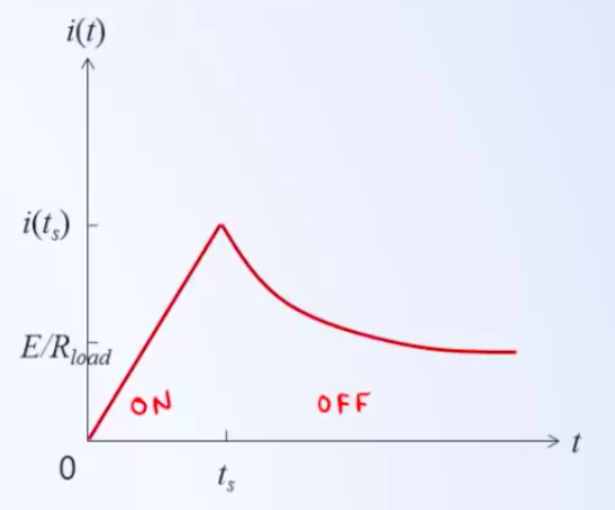
\includegraphics[width=0.75\linewidth]{Bilder/Fund_ELK_Boost_Perforance}
	\caption{Performance of boost converter}
	\label{Fig_Fund_ELK_Boost_Performance}
\end{figure}

When the this ON and OFF states are switched at a certain frequency, the following output current at the battery charging can be observed as shown in figure \ref{Fig_Fund_ELK_Boost_Performance_f}
\begin{figure}[h!]
	\centering
	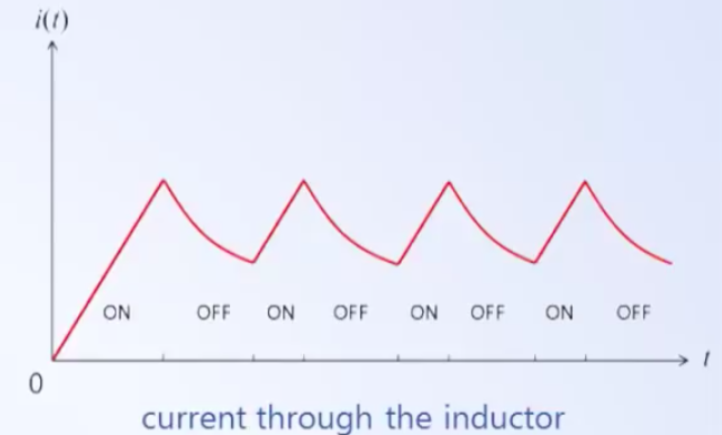
\includegraphics[width=0.75\linewidth]{Bilder/Fund_ELK_Boost_Charging_f}
	\caption{Charging frequency of the boost converter}
	\label{Fig_Fund_ELK_Boost_Performance_f}
\end{figure}
\newpage
The number of charging cycles can be seen as shown in figure \ref{Fig_Fund_ELK_Boost_Charging_Cycles}
\begin{figure}[h!]
	\centering
	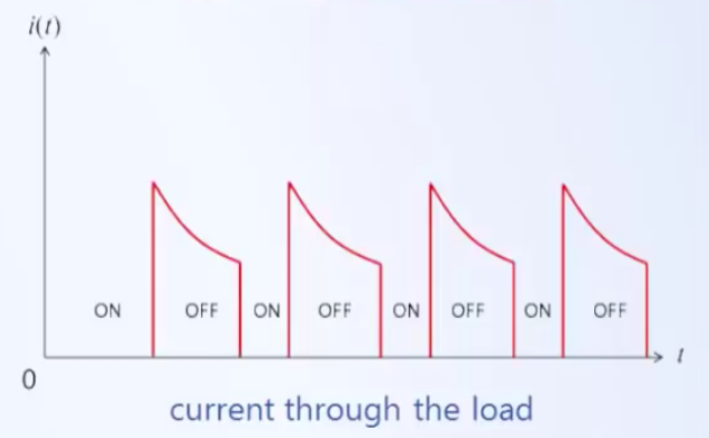
\includegraphics[width=0.75\linewidth]{Bilder/Fund_ELK_Boost_Charging_Cycles}
	\caption{Boost converter charging cycles}
	\label{Fig_Fund_ELK_Boost_Charging_Cycles}
\end{figure}

The variations seen in the charging cycles are generally smoothed out using a capacitor which acts like a low pass filter providing a smooth voltage across the battery. 

\section{Modeling circuits in Laplace Domain}

While modeling circuits in Laplace domain, a quantity can be defined using the ratio between the input voltage and the output current and this quantity is called the complex impedance as described in the following equation:
\begin{equation}
	Z(s) = \frac{E(s)}{I(s)}
\end{equation}

Complex impedance is treated like resistance and therefore can be defined using Ohm's law and using impedance equivalent circuits can be described in series and parallel like we used in resistors. However, impedance is a property of an electrical element that varies with frequency and for each of the electrical element its complex impedance can be described as follows.

\textbf{Resistor}
\begin{equation}
	\mathcal{L}[e = i R] \implies E(s) = I(s)R \implies Z(s) = \frac{E(s)}{I(s)} = R
\end{equation}
In case of resistor impedance is a constant at any input frequencies.

\textbf{Capactor}
\begin{equation}
	\mathcal{L}[e = \frac{1}{C} \int i dt] \implies E(s) = \frac{1}{C} \frac{I(s)}{s} \implies Z(s) = \frac{E(s)}{I(s)} = \frac{1}{Cs}
\end{equation}
Therefore, in case of capacitors the impedance reduces at higher frequencies.

\textbf{Inductors}
\begin{equation}
	\mathcal{L}[e = L \frac{di}{dt}] \implies E(s) = L s I(s) \implies Z(s) = \frac{E(s)}{I(s)} = s L
\end{equation}
Therefore, in case of inductors the impedance increases with the increasing frequency.

\subsection{TF example of voltage divider}

Consider the following circuit as shown in figure \ref{Fig_Fund_ELK_Voltage_Divider}. In this example a method using TF is used to model the circuit instead of time domain modeling done previously using Kirchhoff's Laws.
\begin{figure}[h!]
	\centering
	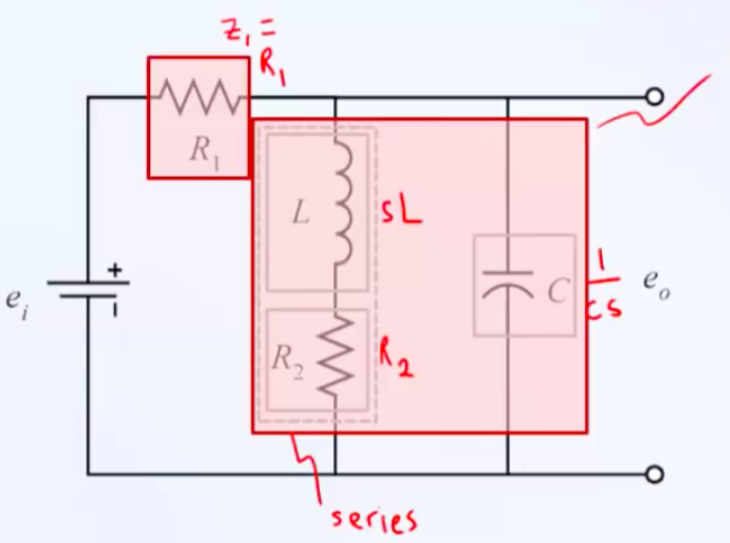
\includegraphics[width=0.75\linewidth]{Bilder/Fund_ELK_Voltage_DIvider}
	\caption{Example for circuit modeling using TF}
	\label{Fig_Fund_ELK_Voltage_Divider}
\end{figure}

The two components $L$ and $R_2$ are in series, as impedance has the same rules as resistors the impedance of these two components can be added up as $$ s L + R_2 $$ further the components in series are parallel to the capacitor, therefore using resistors in parallel formula and calling th whole thing as $Z_2$ as: $$ Z_2 = \left[ \frac{1}{sL + R_2} + \frac{1}{1/Cs} \right]^{-1} $$ Solving the above equation leads to $$ Z_2 = \frac{sL + R_2}{R_1 C L s^2 + (C R_1 R_2 + L)s + R_1 + R_2} $$ Now the system can be seen as a two component system as shown in figure \ref{Fig_Fund_ELK_Voltage_Div_2}
\begin{figure}[h!]
	\centering
	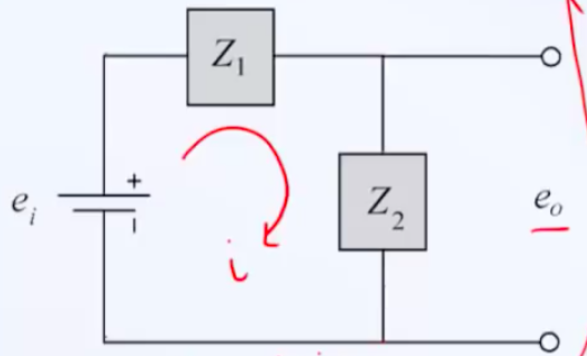
\includegraphics[width=0.75\linewidth]{Bilder/Fund_ELK_Voltage_DIv_2}
	\caption{System modeled in the form representing a voltage divider}
	\label{Fig_Fund_ELK_Voltage_Div_2}
\end{figure}

Using the figure \ref{Fig_Fund_ELK_Voltage_Div_2}, the TF of the system can be written as described, the output voltage is only the voltage across $Z_2$, therefore, the output voltage is defined using resistance law as $$E_{0}(s) = I(s) Z_{2}(s) $$ similarly, the input voltage is the voltage across the two components $Z_1$ and $Z_2$ and is described as: $$ E_{i}(s) = Z_{1}(s)I(s) +  Z_{2}(s)I(s) $$ $I(s)$ cancels out from the equation and substituting $Z_1$ and $Z_2$ in the TF and solving the TF leads to:
\begin{equation}
	G(s) = \frac{sL + R_2}{R_{1} C L s^2 + (C R_{1} R_{2} + L)s + R_1 + R_2}
\end{equation}